% THIS DOCUMENT IS FOLLOWS THE VOLERE TEMPLATE BY Suzanne Robertson and James
% Robertson ONLY THE SECTION HEADINGS ARE PROVIDED
%
% Initial draft from https://github.com/Dieblich/volere
%
% Risks are removed because they are covered by the Hazard Analysis
\documentclass[12pt]{article}

\usepackage{booktabs}
\usepackage{tabularx}
\usepackage{longtable}
\usepackage{hyperref}
\usepackage{graphicx}
\usepackage[center]{caption}
\usepackage{float}
\captionsetup{justification=centering}

\hypersetup{
    bookmarks=true,         % show bookmarks bar?
    colorlinks=true,      % false: boxed links; true: colored links
    linkcolor=red,          % color of internal links (change box color with
    citecolor=green,        % color of links to bibliography
    filecolor=magenta,      % color of file links
    urlcolor=cyan           % color of external links
}

\newcommand{\lips}{\textit{Insert your content here.}}

%% Comments

\usepackage{color}

\newif\ifcomments\commentstrue %displays comments
%\newif\ifcomments\commentsfalse %so that comments do not display

\ifcomments
\newcommand{\authornote}[3]{\textcolor{#1}{[#3 ---#2]}}
\newcommand{\todo}[1]{\textcolor{red}{[TODO: #1]}}
\else
\newcommand{\authornote}[3]{}
\newcommand{\todo}[1]{}
\fi

\newcommand{\wss}[1]{\authornote{blue}{SS}{#1}} 
\newcommand{\plt}[1]{\authornote{magenta}{TPLT}{#1}} %For explanation of the template
\newcommand{\an}[1]{\authornote{cyan}{Author}{#1}}

%% Common Parts

\newcommand{\progname}{Software Engineering} % PUT YOUR PROGRAM NAME HERE
\newcommand{\authname}{Team 21, Alkalytics
\\ Sumanya Gulati - gulats10
\\ Kate Min - mink9
\\ Jennifer Ye - yej52
\\ Jason Tran - tranj78} % AUTHOR NAMES                  

\usepackage{hyperref}
    \hypersetup{colorlinks=true, linkcolor=blue, citecolor=blue, filecolor=blue,
                urlcolor=blue, unicode=false}
    \urlstyle{same}
                                


\begin{document}

\title{Software Requirements Specification for \progname: Alkalytics} 
\author{\authname}
\date{\today}
	
\maketitle

~\newpage

\pagenumbering{roman}

\tableofcontents

~\newpage

\listoffigures
\listoftables

\section*{Volere Template Changes}
\begin{tabularx}{\textwidth}{p{8cm}p{4cm}X} \toprule
  {\textbf{Section Name}} & {\textbf{Action}}\\
  \midrule
  6.3 Work Partioning & Removed\\
  6.4 Specifying a Business Use Case (BUC) & Removed\\
  17.1 and 17.2 & Merged sub-sections\\
  21.3 Planning of the Development Phases & Added\\
  \bottomrule
\end{tabularx}

\newpage
\section*{Revision History}

  \begin{tabularx}{\textwidth}{p{4cm}p{1.5cm}X} \toprule {\textbf{Date}} &
  {\textbf{Version}} & {\textbf{Notes}}\\
  \midrule
  1 October 2024 & 1.0 & Partially completed version shared with supervisors and TA for feedback.\\
  7 October 2024 & 1.1 & Incorporated feedback and presented during informal presentation with TA.\\
  11 October 2024 & 1.2 & Finished document for PoC submission.\\
  11 November 2024 & 1.3 & Updated document to include peer review changes.\\
  \bottomrule
  \end{tabularx}

~\\

~\newpage
\section{Purpose of the Project}
\subsection{User Business}
This project aims to aid in the data management and analysis of an ocean
alkalinity enhancement experiment process. The research is working towards a
scalable process to capture CO\textsubscript{2} using a combination of electric
fields and membranes. The experiment's efficient generation process creates a
very dilute base. As earth’s temperature rises, so does the ocean’s, affects its
pH balance. The experimental study aims to provide a solution, to decrease the
ocean's pH levels to be able to absorb more CO\textsubscript{2} which will in
turn help reduce global temperatures.  As the production process to generate
this dilute base is still on a small scale, it is currently being perfected
which means many more experiments must be done to be able to bring it to a
global scale. However, this requires a massive production operation to do so.
Optimization of the experimental data is critical to improve process efficiency.
This is a big data software problem requiring the ability to find and fine-tune
specific parameters. 
\subsection{Goals of the Project}
This application will be able to consolidate and organize the data from the
experiments with proper labeling across all given datasets allowing for a
centralize method of data storage that is both scalable and maintainable. On the
application users can request to see certain data points from the inputted data
sets given any specified order. Once the data is returned to the user the
application can show inter-parameter comparability to better aid data analysis.
This comparability acts as a starting point to analysis and is by no means show
a final analysis of the data. This will all be presented in a web interface
where all the user functions will be displayed and can be shared among those
involved in the experiment.   
\section{Stakeholders}

\subsection{Client}
Dr. Charles de Lannoy serves as the main client for this project as he is the
lead supervisor of the research study. This solution directly affects his work and
is intended to be a custom solution for the problem. Bassel Abdelkader is
another client of this project as he is the person that works directly with the
research data. One of his responsibilities is to record the experimental data and
upload them to their current data storage system, Microsoft Excel. 
\subsection{Customer}
Since this project is an in-house solution development the inital customer is
also the client. As Dr. Charles de Lannoy is both directing this project and is
also the end user. As such, he is also considered to be the customer.\newline 
Although this project is a tailored solution to one research study, its
application can still be extended to any other situation where large sets of
data is involved. This could be shared among other researchers to aid in their
data management and analysis. Depending on the research team's structure, there
could also be different levels of permissions that can be obtained.
\subsection{Other Stakeholders}
Current student assistants and members of the lab working on the study is can also be
considered stakeholders for the same reasons as the clients. However, since they
will only be working with the study for a short amount of time without daily or
consistent interaction, they do not serve as a main stakeholder. The founder of
the study, who is currently funding the research project is another stakeholder.
However, since they do not work directly with the processes of the study rather
oversee the process, they may not have strong interest in the details of the solution. 
\subsection{Hands-On Users of the Project}
\label{sec:2.4}
The following is a special type of stakeholder as after this capstone project
term, the project will be passed back to the research team to maintain. 
\begin{itemize}
  \item User name/category: Research project team for maintaining this project post capstone 
  \item User Role: Maintain the codebase, adding new features, fixing potential bugs
  project post capstone
  \item Subject matter experience: Master knowledge on the goals of the research
  project. Master knowledge on how the experiment processes work. 
  \item Technical knowledge: Novice knowledge on the technology stack being
  used in this project, Python, MongoDB, JavaScript, other front-end frameworks 
\end{itemize}

\subsection{Personas}
\label{personas}
\begin{itemize}
  \item John Doe is an 23 year old McMaster undergraduate student who has a
  research position on the ocean alkalinity research project. They have been
  tasked to aid the experiment data collection process. After being told that
  the data is being stored in a master Excel file; they find that is it hard to
  use. Being an engineering student without much experience with Excel, they
  struggle to find the data they want. Inputting data is still a manageable
  process but they find themselves to be spending a lot of time looking at Excel
  documentation which they find frustrating as that time could be allocated to
  being more productive during the school term. Although, they want to a better
  way to manage the data, they know that it is not up to their decision on what
  tools are being used but suggested that there could be another better solution
  to use. 
  \item Dr.\ Carly Kelvon is a 60 years old professor at a university and
  is working on her own research project for over five years. She has gathered
  lots of data and thankfully she has always been great at Excel. However, other
  the last two years she has found that Excel is becoming less sustainable. The
  queries are a lot slower and sifting through pages and pages of data is
  wasting a lot of her time. She sees this more evidently through those that
  work along side her as they are also facing the same struggles with even less
  Excel experience as her. She wants to find a more scalable solution but she
  fears that her lack of digital knowledge will do her more harm than good, as a
  result she fears that if she introduces a new application to serve her needs
  better that she will find it hard and confusing to use. 
  \item Dr.\ Alex Stark is a 30 year old associate professor who has recently
  gotten funding for his innovative research idea and has been dedicating all
  his time on perfecting its methodology. It has only been one year since his
  research started but had recently found a great application of his ideas to
  reach far more people and be more impactful that he had originally thought.
  But with his current data management set up, he quickly realises that it is not
  sustainable. He finds that there are many other solutions on the market but
  they do not exactly meet his needs and cost a lot more than what he can spend
  on a tool. He decided that the best way is to create his own tool but lacks
  the software knowledge to create something stable and reliable. 
\end{itemize}
    
\subsection{Priorities Assigned to Users}
\subsubsection{Primary Users}
\begin{itemize}
  \item Dr. Charles de Lannoy
  \item Bassel Abdelkader
  \item Student Assistant working on the experiment 
\end{itemize}

\subsubsection{Secondary Users}
\begin{itemize}
  \item Researcher with their own research studies 
  \item The founder of the study
\end{itemize}
\subsection{User Participation}
Since this project is a personalized solution for a research team, there is no
other user participants other than the research time and others teams with a
similar need. 
\subsection{Maintenance Users and Service Technicians}
Not a relevant section 

\section{Mandated Constraints}
The following constraints highlight the restrictions and limitations imposed by the stakeholders, impacting the implementation of the product. 
\subsection{Solution Constraints}
\textbf{MC-1.} The product must accept Comma-Separated Value (CSV) files as input.
\begin{itemize}
  \item \emph{Rationale}: The lab apparatus generates and stores results as CSV files.
  \item \emph{Fit Criterion}: The product's input process (the processing and acceptance of input data) into the database shall be approved by testers and developers.
\end{itemize}

\subsection{Implementation Environment of the Current System}
\textbf{MC-2.} The product must be able to run on a Windows machine.
\begin{itemize}
  \item \emph{Rationale}: Currently, the lab has a Windows machine that is used to operate the apparatus and analyse the produced results.
  \item \emph{Fit Criterion}: The product shall be approved as Windows compliant by testers and developers.
\end{itemize}

\subsection{Off-the-Shelf Software}
\emph{N/A}

\subsection{Anticipated Workplace Environment}
\textbf{MC-3.} The product shall be used in the Chemical Engineering Lab run by Dr. Charles de Lannoy, Bassel Abdelkader and their team of researchers.

\subsection{Partner or Collaborative Applications}
\emph{N/A}

\subsection{Schedule Constraints}
\textbf{MC-4.} The project must be finished within the course of the current academic year.
\begin{itemize}
  \item \emph{Rationale}: The finished product, as outlined in the project requirements, must be submitted by the end of the academic year.
  A few relevant deadlines include:
  \begin{itemize}
    \item Proof of Concept Demonstration: November 11 to 22, 2024
    \item Revision 0 Demonstration: February 3 to 14, 2025
    \item Final Demonstration (Revision 1): March 24 to 30, 2025
  \end{itemize}
\end{itemize}

\subsection{Budget Constraints}
\textbf{MC-5.} The total cost of the project must not exceed \$750.
\begin{itemize}
  \item \emph{Rationale}: The product must be economically feasible and all teams must have an equal budget to ensure conformity and equality in terms of access of resources.
\end{itemize}

\subsection{Enterprise Constraints}
\emph{N/A}

\section{Naming Conventions and Terminology}
The following are standardized terms used throughout the project and its
documentation to ensure clarity and consistency in communication.

\subsection{Glossary of All Terms, Including Acronyms, Used by Stakeholders Involved in the Project}

\begin{itemize}
    \item \textbf{Alkalinity Enhancement}: A process in ocean engineering to
    increase the ocean's ability to absorb CO\textsubscript{2}.
    \item \textbf{CO\textsubscript{2}}: Carbon Dioxide, a greenhouse gas that
    contributes to global warming.
    \item \textbf{Ion Exchange}: The process of exchanging ions between the
    dilute base and seawater to increase alkalinity.
    \item \textbf{pH Level}: A measure of acidity or alkalinity, critical in
    assessing the effectiveness of the alkalinity enhancement process.
    \item \textbf{Buffering Capacity}: The ability of seawater to resist changes
    in pH, essential for maintaining stable conditions during experiments.
    \item \textbf{Electrodialysis}: A process that uses electric fields to drive
    ion movement through membranes, facilitating the generation of the dilute
    base.
    \item \textbf{Oceans' Carbon Cycle}: The natural process by which carbon is
    exchanged between the ocean, atmosphere, and land, impacting global climate.
    \item \textbf{POC (Proof of Concept)}: A demonstration used to verify that a
    concept is feasible.
    \item \textbf{V\&V (Verification and Validation)}: Ensures that the software
    meets the required standards and performs as expected.
    \item \textbf{CSV (Comma-Separated Values)}: A file format used for storing
    tabular data, such as those from experiments.
    \item \textbf{Data Migration}: The process of transferring data between
    storage types or formats.
    \item \textbf{Backend}: The server side responsible for logic, data
    management, and API services.
    \item \textbf{Frontend}: The user interface built using React, interacting
    with the backend.
    \item \textbf{Database}: A structured storage system (MongoDB) used to
    manage project data.
    \item \textbf{API (Application Programming Interface)}: The means by which
    the frontend communicates with the backend, using GraphQL.
    \item \textbf{CI/CD (Continuous Integration/Continuous Deployment)}:
    Automating testing and deployment to ensure reliable updates.
    \item \textbf{Git}: Distributed version control for tracking code changes
    and enabling collaborative development.
    \item \textbf{Kanban}: A task management method used in to track progress.
    \item \textbf{Branch}: A separate version of the codebase where changes are
    developed.
    \item \textbf{Commit}: A recorded change to the codebase.
    \item \textbf{Pull Request}: A request to merge changes into the main
    codebase after review.
    \item \textbf{Deployment}: Releasing the application to a live environment.
\end{itemize}

\section{Relevant Facts And Assumptions}
External factors that may have an effect on the product have been recorded as relevant facts and assumptions in this section.
\subsection{Relevant Facts}
Currently, two sources of data input are used -
\begin{itemize}
  \item The CSV files that contain datapoints generated by the apparatus.
  \item The initial parameter values for each experiment such as power voltage, age of membrane, density module and more that are inputted into 
  template excel files. These values are manually inputted by the user and remain constant throughout each experiment.
\end{itemize}

\subsection{Business Rules}
\emph{N/A}
\subsection{Assumptions}
\emph{N/A}

\section{The Scope of the Work}
This section determines the boundaries of the project to be studied and outlines how it fits into its environment.
\subsection{The Current Situation}
Currently, a system of excel template files is used to store and manage the data. CSV files are generated by the lab apparatus
which are then downloaded and copied onto an `experiment' excel template. This step involves getting rid of redundant data when a single CSV file is
split into multiple excel files and removing inaccurate data (such as rows of zeroes).\\
\newline
This data in the experiment template is then analysed and the results from the analysis of each experiment is then added to another consolidated excel template,
referred to here as `observations' that reords all experiment observations. This observations template also contains additional parameters for each experiment 
such as membrane, configuration and more wich are entered manually by the user.
\subsection{The Context of the Work}
The path highlighted with blue arrows indicates the current process and how the existing data will be migrated.\\
The path highlighted with green arrows indicates how the product is expected to work after installation.
\begin{figure}[H]
  \centering
  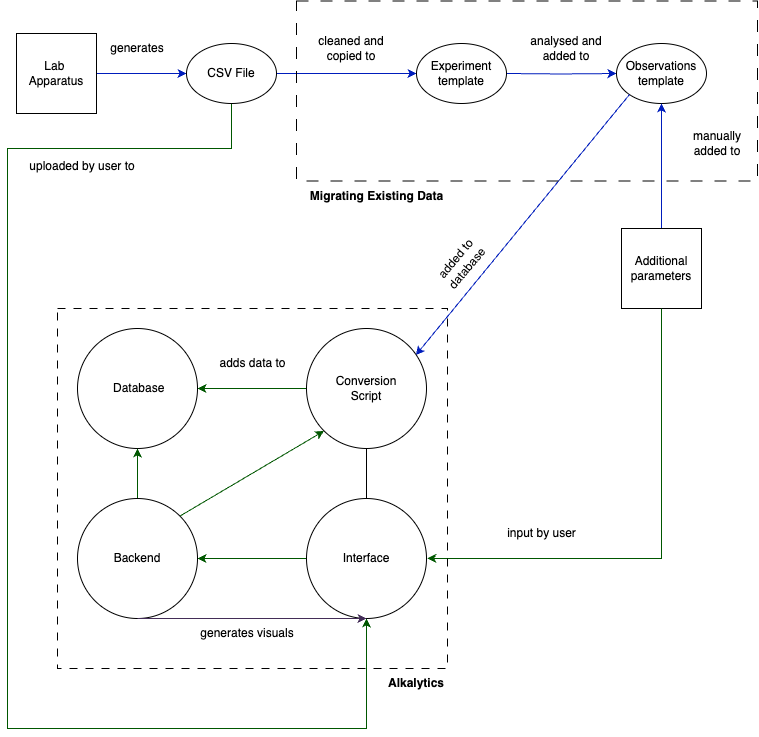
\includegraphics[scale=0.55]{Diagrams/Work Context Diagram.drawio.png}
  \caption{Work Context Model}
\end{figure}

\section{Business Data Model and Data Dictionary}
\subsection{Business Data Model}
The diagram represents a business data model that encapsulates all the data that is
created, referenced, updated and deleted by processes in the platform.

\begin{figure}[H]
  \centering
  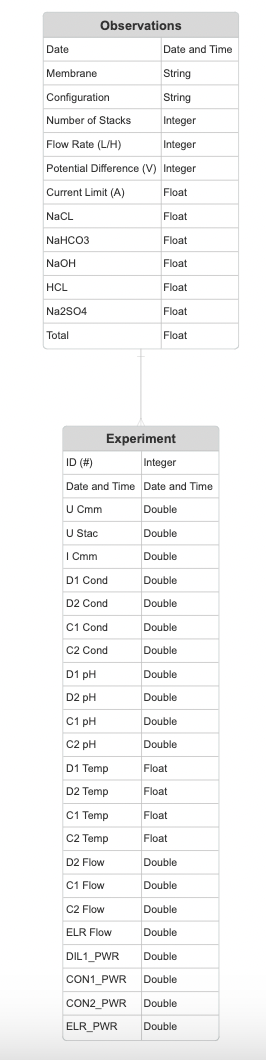
\includegraphics[scale=0.98]{Diagrams/Business Data Model.png}
  \caption{Business Data Model}
\end{figure}

\subsection{Data Dictionary}
\emph{N/A}

\section{The Scope of the Product}
The following section will highlight use cases of the product and how users and
stakeholders will interact with the product.  
\subsection{Product Boundary}
Below is a use case diagram involving the two clients and major customers. The
diagram includes the back end database as an actor as it interacts with the
interface system. Level 1 to 3 labeled actors are part of the research time
customer mentioned in section 2.2 where depending how the team is structured,
there are differnt use cases for different level actors. These are added for
clarity of the system.

\begin{figure}[H]
  \centering
  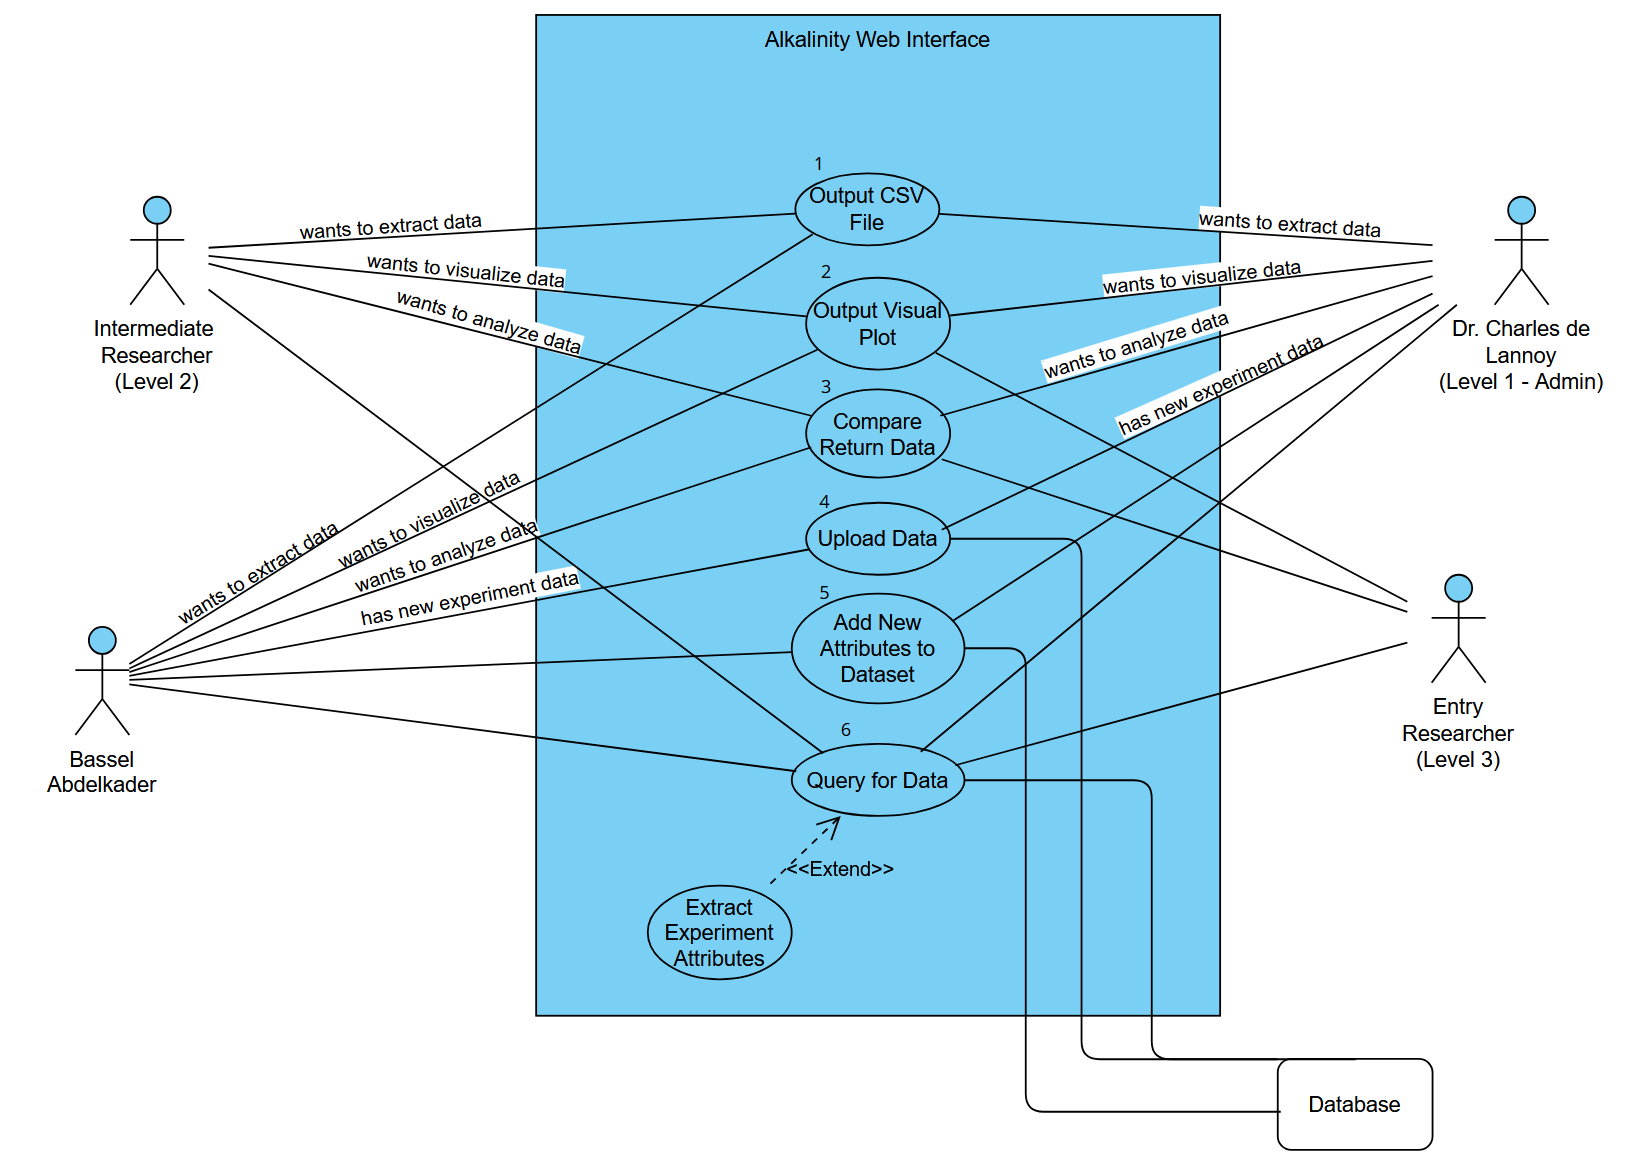
\includegraphics[scale=0.5]{capstoneUseCase.png}
  \caption{Use Case Diagram}
\end{figure}


\subsection{Product Use Case Table}
The product use case table (PUC) is an extention of the use case diagram in the pervious section. The table aims to provide more details.
\begin{table}[htbp]
  \centering
  \begin{tabular}{|p{0.08\linewidth}|p{0.3\linewidth}|l|p{0.4\linewidth}|}
    \hline
    \textbf{PUC No.} & \textbf{PUC Name} & \textbf{Actor/s} & \textbf{Input \& Output}\\
    \hline
    1 & Output CSV& \begin{tabular}[c]{@{}l@{}}Dr.\ Charles de Lannoy\\ Bassel Abdelkader\\ Intermediate Researcher\end{tabular} & \begin{tabular}[c]{@{}l@{}}Downloadable CSV file with\\ appropriate data (out)\\ Success or failure message\\ (out)\end{tabular}                                               \\
    \hline
    2 & Output Visual Plot & \begin{tabular}[c]{@{}l@{}}Dr.\ Charles de Lannoy\\ Bassel Abdelkader\\ Intermediate Researcher\\ Entry Researcher \end{tabular} & \begin{tabular}[c]{@{}l@{}}downloadable portable network\\ graphic (PNG) or portable\\ document format (PDF) file \\(out)\\ Online viewable plot graphic \\(out)\end{tabular}      \\
    \hline
    3 & Compare Return Data & \begin{tabular}[c]{@{}l@{}}Dr.\ Charles de Lannoy\\ Bassel Abdelkader\\ Intermediate Researcher\\ Entry Researcher \end{tabular} & \begin{tabular}[c]{@{}l@{}}Online viewable table of result \\(out)\\ Data analysis results of\\ involved data(out)\end{tabular}                                                \\
    \hline
    4 & Upload Data & \begin{tabular}[c]{@{}l@{}}Dr.\ Charles de Lannoy\\ Bassel Abdelkader\\ Database\end{tabular} & \begin{tabular}[c]{@{}l@{}}CSV file in expected format \\and attributes (in)\\ Success or failure user message \\(out)\\ Update database with inputted\\ data (out)\end{tabular} \\
    \hline
    5 & Add New Attributes to Dataset & \begin{tabular}[c]{@{}l@{}}Dr.\ Charles de Lannoy\\ Bassel Abdelkader\\ Database \end{tabular} & \begin{tabular}[c]{@{}l@{}}Update database with the new \\attribute (out)\\ Success or failure user message \\(out)\\ Attribute name of string type \\(in)\end{tabular}          \\
    \hline
    6 & Query for Data & \begin{tabular}[c]{@{}l@{}}Dr.\ Charles de Lannoy\\ Bassel Abdelkader\\ Intermediate Researcher\\ Entry Researcher\\ Database \end{tabular} & \begin{tabular}[c]{@{}l@{}}Visual online table with the \\queried data (out)\\ Selected attribute(s), dates,\\ restrictions (in)\end{tabular}\\
    \hline
    \end{tabular}
    \caption{Product Use Cases}
\end{table}  


\newpage  \subsection{Individual Product Use Cases (PUC's)}
\subsubsection{Output CSV}
\begin{itemize}
  \item Description: The user can export/output the data that they have received
  from any function on the website system
  \item Pre-condition: There must be some data in the database. The information
  the user wants to output must also be able to be stored in a CSV file 
  \item Post-condition: The user will get to download the desired CSV file
  containing data from the database. If the download file has been sent to the
  system, the user will receive a success or failure message.
  \item Basic path: After querying the data from the database is successful, the
  user can click on the download CSV button to export the file onto their system.
\end{itemize}

\subsubsection{Output Visual Plot}
\begin{itemize}
  \item Description: The user is able to generate a graphical plot based on data
  from the database. The contents of the graph can be customized to include any
  sort of data that the user decides from the data base. The graph type can be determined by the user. 
  \item Pre-condition: There must be some selected data to be used to plot a graph.
  \item Post-condition: A online view of the plot will be generated and
  displayed on the website. There will also be an option for downloadable version. 
  \item Basic path: After querying the database for desired data, the user can
  pick the option to plot the returned data. The website will then generate a
  graphical plot based on the returned data.
\end{itemize}

\subsubsection{Compare Return Data}
\begin{itemize}
  \item Description: This use case will allow the user to compare two sets of
  data such as differences or similarities among other criteria.
  \item Pre-condition: There must be two sets of data and what attribute(s) are
  being compared. 
  \item Post-condition: The analysis of the data will be presented in a visual
  manner. Possible outcome may include colour coded elements or a small statement. 
  \item Basic path: After querying the database for desired data, the user can
  choose to enable the compare function. The user will then need to pick what
  attributes they would like to compare and then continue with the website
  prompts which will eventually give the data analysis result.
\end{itemize}

\subsubsection{Upload Data}
\begin{itemize}
  \item Description: When the user has more experimental data and would like to
  update the database, this function of the website will be used to take in the
  data and update/add to the existing database.
  \item Pre-condition: The file with the new data will be a CSV file and will
  need to be uploaded through the website interface.
  \item Post-condition: A success or failure message will be displayed to the
  user once the file is done uploading and have been added to the database.
  \item Basic path: The user will need to click on the upload data button and
  find the file they wish to upload on their system and upload it through the
  website's drop box. 
\end{itemize}
\subsubsection{Add New Attributes to Dataset}
\begin{itemize}
  \item Description: As the experiment and data become larger or changes have
  been made, there will be times when the dataset will need to be changed by
  adding new attributes.  
  \item Pre-condition: The user must specify which dataset that they want to
  edit. The user must then specify what is the attribute name is in the form of
  a string type input. 
  \item Post-condition: A success or failure message will be displayed to the
  user once the new attribute has been added to the database. 
  \item Basic path: The user will need to click on the edit dataset button. The
  user must then fill in the input fields with the correct information
\end{itemize}

\subsubsection{Query for Data}
\begin{itemize}
  \item Description: The user will want to get data from their past experiments.
  To do so, they will need to decide what they want. This is one of the main use
  case for any user/actor. 
  \item Pre-condition: The database must have the some data. The user's query
  request must be filled in through the input fields. The fields can range from
  dates, to strings, to constraints. 
  \item Post-condition: The returned data will be shown to the user through a
  visual table representation and will be presented with a range of other
  functions that the user can do with the returned data.  
  \item Basic path: The user will need to click on the query function button.
  They will then need to fill in the input fields, go through the user prompts
  to then get the output.
\end{itemize}

\section{Functional Requirements}
This section outlines the key functionalities the application must satisfy with justifications and fit criteria, as well as proposed phase-in dates.
\subsection{Data Input Requirements}
  \begin{enumerate}
    \item[\textbf{FR-1.}] The application shall allow the user to input new experiment data or parameters.
    \begin{itemize}
    \item \textit{Rationale}: The application needs to be kept up-to-date with ongoing experiments, which may include new parameters that did not exist previously.
    \item \textit{Fit Criterion}: The user should be able to input new data and parameters without any errors.
    \item \textit{Priority}: Medium; This is dependent on having FR-2 implemented and can be developed later on.
    \item \textit{Phase-in Date}: Jan 17.
    \item \textit{Related Requirements}: FR-2, PR-1, PR-14, SR-3.
    \end{itemize}
    \item[\textbf{FR-2.}] The application shall store experiment data in the database with all associated parameters and values correctly labelled.
    \begin{itemize}
      \item \textit{Rationale}: Ensures that data retrieval and analysis will be correct and accurate.
      \item \textit{Fit Criterion}: The application's database parameters and values shall match the original experiment data parameters and values.
      \item \textit{Priority}: High; This is part of the functionalities that must be implemented for the proof of concept demonstration.
      \item \textit{Phase-in Date}: Nov 10.
      \item \textit{Related Requirements}: UHR-3, FR-1, FR-4, FR-5, FR-6, FR-8, FR-10, FR-11, PR-1, PR-6, PR-7, PR-12, PR-13, SR-3.
    \end{itemize}
  \end{enumerate}

\subsection{Data Migration and Organization Requirements}
  \begin{enumerate}
    \item[\textbf{FR-3.}] The application shall read existing experiment data stored in .CSV files.
    \begin{itemize}
      \item \textit{Rationale}: Existing experiment data is stored in Excel spreadsheets and must be integrated into the new application for continuity and analysis.
      \item \textit{Fit Criterion}: The application shall read and import the data files without any errors.
      \item \textit{Priority}: High; This is part of the functionalities that must be implemented for the proof of concept demonstration.
      \item \textit{Phase-in Date}: Nov 10.
      \item \textit{Related Requirements}: PR-12, SR-4, SR-5, SR-6.
    \end{itemize}
    \item[\textbf{FR-4.}] The application shall organize experiment data by timestamps and experiment ID for unique identification.
    \begin{itemize}
      \item \textit{Rationale}: Each experiment needs to be separately identified for quick retrieval of data and efficiency in search or query actions.
      \item \textit{Fit Criterion}: Each ID and timestamp shall be traceable to one experiment.
      \item \textit{Priority}: High; This is part of the functionalities that must be implemented for the proof of concept demonstration.
      \item \textit{Phase-in Date}: Nov 10.
      \item \textit{Related Requirements}: FR-2, PR-7, FR-5, FR-6, FR-8, MSR-3, SR-3, SR-4, SR-5, SR-6.
    \end{itemize}
  \end{enumerate}

\subsection{Data Search and Query Requirements}
\begin{enumerate}
  \item[\textbf{FR-5.}] The application shall allow the user to search for specific datasets based on different parameters.
  \begin{itemize}
    \item \textit{Rationale}: The user must be able to do quick look-ups of certain experiments and their results.
    \item \textit{Fit Criterion}: The application shall retrieve the correct experiments based on the matching parameters.
    \item \textit{Priority}: High; This is part of the functionalities that must be implemented for the proof of concept demonstration.
    \item \textit{Phase-in Date}: Nov 10.
    \item \textit{Related Requirements}: FR-2, FR-4, PR-6, FR-7, FR-10, PR-2.
  \end{itemize}
  \item[\textbf{FR-6.}] The application shall allow the user to query two or more parameters or datasets for comparison and analysis.
  \begin{itemize}
    \item \textit{Rationale}: Allows for direct comparisons between different experiment parameters and/or results, which is necessary for data analysis.
    \item \textit{Fit Criterion}: The application shall retrieve the correct parameters and/or experiments based on the query inputs.
    \item \textit{Priority}: High; This is one of the first functionalities that must be implemented for the proof of concept demonstration.
    \item \textit{Phase-in Date}: Nov 10.
    \item \textit{Related Requirements}: FR-2, FR-4, PR-6, FR-7, FR-10, FR-11, FR-15, PR-2.
  \end{itemize}
  \item[\textbf{FR-7.}] The application shall display the results of a user’s selected search or query in a format that is readable to the user.
  \begin{itemize}
    \item \textit{Rationale}: The user needs to see the results in a format that they can interpret.
    \item \textit{Fit Criterion}: The results shall be displayed in a table with all labels correct and legible.
    \item \textit{Priority}: Medium; Its implementation depends on the successful implementation of several other requirements, thus will be properly implemented at a later time.
    \item \textit{Phase-in Date}: Jan 17.
    \item \textit{Related Requirements}: FR-5, FR-6, PR-3, PR-10.
  \end{itemize}
\end{enumerate}

\subsection{Data Visualization Requirements}
\begin{enumerate}
  \item[\textbf{FR-8.}] The application shall generate visual graphs based on selected parameters and datasets.
  \begin{itemize}
    \item \textit{Rationale}: Visual representation of the data allows for easy interpretation and graphical analysis.
    \item \textit{Fit Criterion}: The result should display a graphical plot with a title, axes, labels, and a legend.
    \item \textit{Priority}: Medium; Although this is a core functionality for the application, its implementation depends on the successful implementation of several other requirements, thus will be properly implemented at a later time.
    \item \textit{Phase-in Date}: Jan 17.
    \item \textit{Related Requirements}: FR-2, FR-4, FR-9, LFR-4, PR-5, PR-8, PR-10.
  \end{itemize}
  \item[\textbf{FR-9.}] The application shall allow the user to customize the data visualization by adjusting axes, data ranges, labels, etc.
  \begin{itemize}
    \item \textit{Rationale}: Allows the user to adjust the graphical representation to their needs for their analysis.
    \item \textit{Fit Criterion}: Modifications to axes, data ranges, labels should be reflected in the generated graph in real-time.
    \item \textit{Priority}: Low; This depends on the successful implementation of FR-8 and thus will be implemented at a later time.
    \item \textit{Phase-in Date}: March 21.
    \item \textit{Related Requirements}: FR-8.
  \end{itemize}
\end{enumerate}

\subsection{Data Analysis Requirements}
\begin{enumerate}
    \item[\textbf{FR-10.}] The application shall analyze patterns and trends in the experiment data based on the user’s selected parameters.
    \begin{itemize}
      \item \textit{Rationale}: Trend analysis is critical for the user to discover important findings pertaining to the experiment.
      \item \textit{Fit Criterion}: The application shall generate a result of the analysis to display to the user.
      \item \textit{Priority}: Medium; Although this is a core functionality for the application, its implementation depends on the successful implementation of many other requirements and thus will be implemented at a later time.
      \item \textit{Phase-in Date}: Jan 17.
      \item \textit{Related Requirements}: FR-2, FR-5, FR-6, PR-6, FR-11.
    \end{itemize}
    \item[\textbf{FR-11.}] The application shall use machine learning algorithms to predict and interpolate the data.
    \begin{itemize}
      \item \textit{Rationale}: Allows for future predictions of data and efficiency when designing future experiments.
      \item \textit{Fit Criterion}: The application shall generate a report of value predictions or interpolate a graph and provide the interpolated data points.
      \item \textit{Priority}: Medium; Although this is a core functionality for the application, its implementation depends on the successful implementation of many other requirements and thus will be implemented at a later time.
      \item \textit{Phase-in Date}: Jan 17.
      \item \textit{Related Requirements}: FR-2, FR-6, FR-10, PR-6.
    \end{itemize}
\end{enumerate}

\subsection{Error Tracking Requirements}
This section outlines functional requirements for one of the project's stretch
goals.
\begin{enumerate}
  \item[\textbf{FR-12.}] The application shall track and log errors in the experiment data.
  \begin{itemize}
    \item \textit{Rationale}: Users need to identify irrelevant or missing parameters.
    \item \textit{Fit Criterion}: Missing values in the input data should be flagged.
    \item \textit{Priority}: Low; As this is part of the stretch goals for the application, its implementation will not be considered until all higher priority requirements are satisfied.
    \item \textit{Phase-in Date}: March 21.
    \item \textit{Related Requirements}: FR-13, MSR-3, MSR-5, SR-9.
  \end{itemize}
  \item[\textbf{FR-13.}] The application shall remove data logged as errors.
  \begin{itemize}
    \item \textit{Rationale}: Ensures data is organized and produces accurate results in analysis.
    \item \textit{Fit Criterion}: Flagged data should be removed from the database by the algorithm.
    \item \textit{Priority}: Low; As this is part of the stretch goals for the application, its implementation will not be considered until all higher priority requirements are satisfied.
    \item \textit{Phase-in Date}: March 21.
    \item \textit{Related Requirements}: FR-12, SR-9.
  \end{itemize}
\end{enumerate}

\subsection{User Access Management Requirements}
This section outlines functional requirements for one of the project's stretch
goals.
\begin{enumerate}
  \item[\textbf{FR-14.}] The application shall allow the user to sign in with valid credentials.
  \begin{itemize}
    \item \textit{Rationale}: Ensures the data can only be accessed and modified by authorized users.
    \item \textit{Fit Criterion}: The user shall be able to log in with a username and password.
    \item \textit{Priority}: Medium; Although this requirement is part of the
    stretch goals for the application, its implementation is prioritized over
    the other stretch goals as role-based access control is critical for
    preventing unauthorized modifications and ensuring the integrity of the
    associated data.
    \item \textit{Phase-in Date}: Jan 17.
    \item \textit{Related Requirements}: PR-11, SR-1, SR-2, SR-8, SR-10, SR-11.
  \end{itemize}
\end{enumerate}

\subsection{Data Export Requirements}
This section outlines functional requirements for one of the project's stretch
goals.
\begin{enumerate}
  \item[\textbf{FR-15.}] The application shall generate a report of queries in a session for the user to save or download.
  \begin{itemize}
    \item \textit{Rationale}: Allows user to keep a record of their findings for future use or reference.
    \item \textit{Fit Criterion}: The report should be exported in CSV or PDF format.
    \item \textit{Priority}: Low; As this is part of the stretch goals for the application, its implementation will not be considered until the higher priority requirements are satisfied.
    \item \textit{Phase-in Date}: March 21.
    \item \textit{Related Requirements}: FR-6.
  \end{itemize}
\end{enumerate}

\section{Look and Feel Requirements}
This section will highlight the look and feel of the web interface for the
project involving the appearance and the style of the user interface and
experience.
\subsection{Appearance Requirements}
\begin{enumerate}
  \item[\textbf{LFR-1.}] The website should have a simple and organized layout, with
  clearly defined sections where all major functions should be easily accessible
  and viewable.
  \begin{itemize}
    \item \textit{Rationale:} Having a simple organized layout will ensure that the
    navigation of the website is quick and intuitive for accessing features and
    functions, which will enhance the user experience.
    \item \textit{Fit Criterion:} A user should be able to identify all the major
    functions of the website within five minutes of use.
  \end{itemize}
  
  \item[\textbf{LFR-2.}] The website shall be responsive on all computer and laptop screens
  aside from mobile screens.
  \begin{itemize}
    \item \textit{Rationale:} Having a responsive website will ensure that the
    application accommodates the majority, if not all, of the user base in having a
    proper user experience. 
    \item \textit{Fit Criterion:} The usability of the website should be the same
    as the default view on larger and smaller computer, laptop, and monitor screens.
  \end{itemize}
  
  \item[\textbf{LFR-3.}] The website's functions and buttons shall be properly labeled
  so that no button is ambiguous to users.
  \begin{itemize}
    \item \textit{Rationale:} Limiting ambiguity will ensure that users
    understand and recognize the functions to minimize confusion and improve
    efficiency.
    \item \textit{Fit Criterion:} A user should be able to tell what all buttons
    inherently do without needing to ask questions.
  \end{itemize}
  
  \item[\textbf{LFR-4.}] The produced plot from the data shall be properly labeled.
  \begin{itemize}
    \item \textit{Rationale:} Properly labeling plots will help users
    accurately interpret the data to make important analytical understandings.
    \item \textit{Fit Criterion:} The plots should not be ambiguous; users
    should be able to understand what the plot is about within five minutes of
    viewing it.
  \end{itemize}
\end{enumerate}


\subsection{Style Requirements}
\begin{enumerate}
  \item[\textbf{LFR-5.}] All icons on the website must be in the design standard. 
  \begin{itemize}
    \item \textit{Rationale:} To enforce an identity and unity for the website. 
    \item \textit{Fit Criterion:} After a user's first encounter with the product, 90\% of users should
    see that there is unity among all the icons on the website. 
  \end{itemize}
  
  \item[\textbf{LFR-6.}] All colors must match the theme of the website.
  \begin{itemize}
    \item \textit{Rationale:} Applying a theme will ensure users have
    an engaging visual experience.
    \item \textit{Fit Criterion:} After a user's first encounter with the product, 80\% of users
    should agree that there is a common theme throughout the website.
  \end{itemize}
  
  \item[\textbf{LFR-7.}] All fonts are to be consistent throughout the website. 
  \begin{itemize}
    \item \textit{Rationale:} Consistent fonts will increase readability,
    ensuring users can focus on the functionalities that matter on the page rather than inconsistencies. 
    \item \textit{Fit Criterion:} After a user's first encounter with the product, there should
    be no user who feels that any fonts do not belong on the website. 
  \end{itemize}
\end{enumerate}

\section{Usability and Humanity Requirements}
This section outlines the requirements that are intended to make the product usable and ergonomically acceptable to its users.
\subsection{Ease of Use Requirements}
\textbf{UHR-1.} The product must be easy to navigate and use for 85\% of individuals with basic computer literacy.
\begin{itemize}
  \item \emph{Rationale}: The product must be user-friendly. In the context of this project, basic computer literacy is defined to encompass five computer skills - using a keyboard
  to type, using a mouse to navigate, understanding basic software applications such as word processing and spreadsheets, browsing the internet, and managaing files and folders.
  \item \emph{Fit Criterion}: An individual with basic computer literacy, such as John Doe as described in \nameref{personas} must be able to launch the application and upload an input file
  without any assistance from the administrator.
\end{itemize}

\subsection{Personalization and Internationalization Requirements}
\textbf{UHR-2.} The current version of the product will only be available in English (EN-US) and more languages can be added in the later versions.
\begin{itemize}
  \item \emph{Rationale}: Currently, the product is only expected to be used by McMaster faculty and staff who are fluent in English.
\end{itemize}
\bigskip
\textbf{UHR-3.} The product must recognize commonly used scientific and mathematical symbols.
\begin{itemize}
  \item \emph{Rationale}: The product shall be used to store scientific parameters as datapoints so the product must be able to recognize commonly used symbols used to specify scientific properties.
  \item \emph{Fit Criterion}: The product must be able to recognize the uppercase and lowercase Greek Alphabet.
\end{itemize}

\subsection{Learning Requirements}
\textbf{UHR-4.} 85\% of users must be able to use the product without any formal training and with minimal guidance.
\begin{itemize}
  \item \emph{Rationale}: The product shall be intuitive to use. Users must be able to freely naviagte and experiment with the product after a simple product walkthrough.
  \item \emph{Fit Criterion}: A new user with basic computer literacy skills should be able to upload an input file, enter initial experiment parameters, select fields to be compared and view their graph
  after a simple product walkthrough by the administrator.
\end{itemize}

\subsection{Understandability and Politeness Requirements}
\textbf{UHR-5.} The product shall maintain consistent use of terminology across the platform to avoid confusion.
\begin{itemize}
  \item \emph{Rationale}: As an example, if the term "parameters" has been used in one part of the interface, it will not be used interchangeably with "variables" in a different part of the interface.
  \item \emph{Fit Criterion}: A thorough visual inspection conducted by testers should not reveal any discrepancies.
\end{itemize}

\subsection{Accessibility Requirements}
\textbf{UHR-6.} The web interface of the product must be fully compliant with the Web Content Accessibility Guidelines (WCAG) 2.1 standards at Level AA.
\begin{itemize}
  \item \emph{Rationale}: WCAG 2.1, Level AA compliance is an internationally accepted, common standard for making web content more accessible.
  \item \emph{Fit Criterion}: Compliance with the standard will be tested by testers and measured using the Level AA compliance checklist.
\end{itemize}

\section{Performance Requirements}
Performance requirements define the measurable standards the application must meet regarding speed, accuracy, robustness, and resource usage to ensure optimal performance of the application's functions.
\subsection{Speed and Latency Requirements}
\begin{enumerate}
\item[\textbf{PR-1.}] The application shall store new data or parameters within 60 seconds of input.
  \begin{itemize}
    \item \textit{Rationale}: The speed at which the task can be completed depends on the size of the new data to be inputted or how the addition of a new parameter will affect the existing database structure. The quantified timeframe allows for adequate processing time that aligns with user expectations.
    \item \textit{Related Requirements}: FR-1, FR-2.
  \end{itemize}
\item[\textbf{PR-2.}] The application shall take a maximum of 3 seconds to retrieve data from the database for search and query requests.
  \begin{itemize}
    \item \textit{Rationale}: The speed at which the task can be completed varies based on internet connectivity and the complexity of the query being executed.
    \item \textit{Related Requirements}: FR-5, FR-6.
  \end{itemize}
\item[\textbf{PR-3.}] The interaction between the interface and the user shall have an average response time of 1 second under stable internet connection.
  \begin{itemize}
    \item \textit{Rationale}: Ensures a fluid interaction between the user and the application.
    \item \textit{Related Requirements}: FR-7.
  \end{itemize}
\item[\textbf{PR-4.}] The application shall have a maximum latency of 2 seconds for search and query actions.
  \begin{itemize}
    \item \textit{Rationale}: Ensures that the delay between a user's request and the application's response is minimized to provide the user with quick feedback and a smoother user experience.
  \end{itemize}
\item[\textbf{PR-5.}] The application shall generate visualizations of data in an average time of 10 seconds, depending on the size of the dataset being processed.
  \begin{itemize}
    \item \textit{Rationale}: The time required to render a graph will be affected by the number of datapoints included in the plot. Larger datasets will take longer to process and display.
    \item \textit{Related Requirements}: FR-8.
  \end{itemize}
\end{enumerate}
\begin{itemize}
  \item \textit{Fit Criteria for PR-1 to PR-5}: The application shall satisfy the requirements above.
\end{itemize}

\subsection{Safety-Critical Requirements}
N/A; the application does not have safety-critical requirements to consider.

\subsection{Precision or Accuracy Requirements}
\begin{enumerate}
  \item[\textbf{PR-6.}] All parameter values shall be accurate to four decimal places.
    \begin{itemize}
      \item \textit{Related Requirements}: FR-2, FR-5, FR-6, FR-10, FR-11.
    \end{itemize}
  \item[\textbf{PR-7.}] All timestamps of experiment data shall be accurate to milliseconds.
    \begin{itemize}
      \item \textit{Related Requirements}: FR-2, FR-4.
    \end{itemize}
  \item[\textbf{PR-8.}] Values on visual data plots shall be accurate to four decimal places.
    \begin{itemize}
        \item \textit{Related Requirements}: FR-8.
    \end{itemize}
\end{enumerate}
\begin{itemize}
  \item \textit{Rationales for PR-6 to PR-8}: Accuracy of the data is critical for data analysis, prediction, and interpolation.
  \item \textit{Fit Criteria for PR-6 to PR-8}: The application shall satisfy the requirements above.
\end{itemize}

\subsection{Robustness or Fault-Tolerance Requirements}
\begin{enumerate}
  \item[\textbf{PR-9.}] The application shall not crash but display an error message if it loses connection to the backend server.
  \item[\textbf{PR-10.}] The application shall not terminate but allow the user to view previously loaded queries and generated plots if it loses connection to the internet.
\end{enumerate}
\begin{itemize}
  \item \textit{Rationales for PR-9 and PR-10}: The application should not fail or crash when experiencing unexpected circumstances.
  \item \textit{Related Requirements}: FR-7, FR-8.
\end{itemize}

\subsection{Capacity Requirements}
\begin{enumerate}
  \item[\textbf{PR-11.}] The application shall allow for up to three simultaneous users.
    \begin{itemize}
      \item \textit{Rationale}: The number of anticipated end-users is currently three.
      \item \textit{Related Requirements}: FR-14.
    \end{itemize}
  \item[\textbf{PR-12.}] The application shall be capable of storing data for up to 300 experiments.
    \begin{itemize}
      \item \textit{Rationale}: The application must be capable of storing and processing large amounts of data.
      \item \textit{Related Requirements}: FR-2, FR-3, PR-13.
    \end{itemize}
\end{enumerate}
\begin{itemize}
  \item \textit{Fit Criteria for PR-11 and PR-12}: The application shall satisfy the requirements above.
\end{itemize}

\subsection{Scalability or Extensibility Requirements}
\begin{enumerate}
  \item[\textbf{PR-13.}] The application shall be able to process and store the existing data. The amount of data going into the application is expected to grow until the experiment study comes to an end.
    \begin{itemize}
      \item \textit{Related Requirements}: FR-2, PR-12, PR-15.
    \end{itemize}
  \item[\textbf{PR-14.}] The application shall be able to add additional parameters that did not previously exist in the database at the discretion of the user.
    \begin{itemize}
      \item \textit{Related Requirements}: FR-1, PR-15.
    \end{itemize}
\end{enumerate}
\begin{itemize}
  \item \textit{Rationales for PR-13 and PR-14}: The application must be able to expand to keep up with future experiments.
\end{itemize}

\subsection{Longevity Requirements}
\begin{enumerate}
  \item[\textbf{PR-15.}] The application shall operate for the duration of the experiment study.
  \begin{itemize}
    \item \textit{Related Requirements}: PR-13, PR-14.
  \end{itemize}
\end{enumerate}

\section{Operational and Environmental Requirements}
Operational requirements outline the conditions in which the application is expected to operate, which includes system compatibility and distribution requirements.
\subsection{Expected Physical Environment}
\begin{enumerate}
  \item[\textbf{OER-1.}] The application shall operate in a typical lab environment with reliable internet connectivity.
    \begin{itemize}
      \item \textit{Rationale}: Ensures functionality in environments where end-users are most likely to use the application. 
      \item \textit{Related Requirements}: MC-1
    \end{itemize}
\end{enumerate}

\subsection{Wider Environment Requirements}
\begin{enumerate}
  \item[\textbf{OER-2.}] The application shall be compatible with desktop environments running Windows.
    \begin{itemize}
      \item \textit{Rationale}: Ensures functionality in the technological environment the product is expected to run on.
      \item \textit{Fit Criterion}: Testing will be conducted on the Windows operating system.
      \item \textit{Related Requirements}: MC-2
    \end{itemize}
\end{enumerate}

\subsection{Requirements for Interfacing with Adjacent Systems}
\begin{enumerate}
  \item[\textbf{OER-3.}] The application shall operate on the most recent versions of Chromium-based web browsers.
    \begin{itemize}
      \item \textit{Rationale}: The application should be compatible with Chromium-based web browsers to ensure broad availability and smooth operation on widely-used platforms by the end-users.
      \item \textit{Fit Criterion}: Performance testing shall be done to ensure the application functions correctly.
    \end{itemize}
\end{enumerate}

\subsection{Productization Requirements}
\begin{enumerate}
  \item[\textbf{OER-4.}] The application shall be distributed as a web application.
    \begin{itemize}
      \item \textit{Rationale}: Ensures easy access and usability for the end-users who do not have enough experience in database management.
    \end{itemize}
  \item[\textbf{OER-5.}] The application shall have an easy onboarding process with user documentation.
    \begin{itemize}
      \item \textit{Rationale}: Ensures that users can use the application without needing frequent external support.
      \item \textit{Fit Criterion}: Usability testing shall be done to ensure users are able to onboard easily.
    \end{itemize}
\end{enumerate}

\subsection{Release Requirements}
\begin{enumerate}
  \item[\textbf{OER-6.}] The first version of the application shall be released after project completion.
    \begin{itemize}
      \item \textit{Related Requirements}: MC-4.
    \end{itemize}
\end{enumerate}

\section{Maintainability and Support Requirements}
Maintenance requirements encompass the strategies and processes needed to ensure
a system remains functional, efficient, and up-to-date throughout its lifecycle.

\subsection{Maintenance Requirements}
\begin{enumerate}
  \item[\textbf{MSR-1.}] The application’s maintenance must be the
  responsibility of the development team with no involvement from the users.
  \begin{itemize}
    \item \textit{Rationale:} Ensures that skilled personnel handle maintenance.
  \end{itemize}

  \item[\textbf{MSR-2.}] Documentation must be provided to be referenced for
  future maintenance and to enable seamless knowledge transfer to a new team.
  \begin{itemize}
    \item \textit{Rationale:} Ensures smooth onboarding and continuity in
    development.
    \item \textit{Fit Criterion:} The documentation must be updated with every
    major release.
    \item \textit{Related Requirements:} MSR-3.
  \end{itemize}

  \item[\textbf{MSR-3.}] The application must be designed to accommodate future
  development, including the addition of new experimental parameters or features
  without backwards progression.
  \begin{itemize}
    \item \textit{Rationale:} Ensures the application can scale and evolve
    without compromising existing features.
    \item \textit{Related Requirements:} FR-4, FR-12, MSR-2.
  \end{itemize}
\end{enumerate}

\subsection{Supportability Requirements}
\begin{enumerate}
  \item[\textbf{MSR-4.}] 
  The application must have an intuitive user interface that allows users to
  operate it independently without requiring external assistance.
  \begin{itemize}
    \item \textit{Rationale:} Ensures a user-friendly experience that reduces
    the need for help desk support.
    \item \textit{Fit Criterion:} At least 90\% of users should be able to
    complete tasks without needing support.
    \item \textit{Related Requirements:} LF-1, LF-2, LF-3, UHR-1, UHR-4.
  \end{itemize}

  \item[\textbf{MSR-5.}] The application must have automated guidance, such as
  error messages, to assist users in troubleshooting common issues.
  \begin{itemize}
    \item \textit{Rationale:} Ensures users can resolve issues on their own,
    reducing the volume of support requests.
    \item \textit{Fit Criterion:} The documentation must be updated with every
    major release and reviewed quarterly to ensure accuracy.
    \item \textit{Related Requirements:} FR-12.
  \end{itemize}
\end{enumerate}

\subsection{Adaptability Requirements}
\begin{enumerate}
  \item[\textbf{MSR-6.}] The application must be compatible with modern web
  browsers to ensure widespread accessibility.
  \begin{itemize}
    \item \textit{Rationale:} Ensures the application is accessible to a broad
    range of users and devices.
    \item \textit{Fit Criterion:} The application should at least be able to run
    on the latest version of Chromium-based web browsers.
    \item \textit{Related Requirements:} LF-1, LF-2.
  \end{itemize}
\end{enumerate}
\section{Security Requirements}
Security requirements focus on protecting data, controlling access, ensuring
integrity, and auditing user actions within the application.

\subsection{Access Requirements}
\begin{enumerate}
  \item[\textbf{SR-1.}] Access to the application must be restricted to
  authorized personnel, with an authentication mechanism.
  \begin{itemize}
    \item \textit{Rationale:} Ensures that only authorized users can interact
    with the application.
    \item \textit{Fit Criterion:} Only users with valid credentials should
    access the application.
    \item \textit{Related Requirements:} FR-14, SR-2, SR-8, SR-10.
  \end{itemize}

  \item[\textbf{SR-2.}] Only authenticated users should have the ability to
  query or modify the data, and each user’s access must be limited to their
  capabilities within the application.
  \begin{itemize}
    \item \textit{Rationale:} Ensures users can only perform actions that align
    with their roles.
    \item \textit{Fit Criterion:} The application should restrict 100\% of
    actions that are not permitted to the user's level of access.
    \item \textit{Related Requirements:} FR-14, SR-1, SR-8.
  \end{itemize}
\end{enumerate}

\subsection{Integrity Requirements}
\begin{enumerate}
  \item[\textbf{SR-3.}] The application must validate data inputs to ensure they
  conform to expected formats and values before they are processed.
  \begin{itemize}
    \item \textit{Rationale:} Ensures only valid data is processed, reducing
    errors.
    \item \textit{Fit Criterion:} 100\% of inputs must pass validation checks
    before processing.
    \item \textit{Related Requirements:} FR-1, FR-2, FR-4.
  \end{itemize}

  \item[\textbf{SR-4.}] The application must not modify the data unnecessarily
  through its transfer process.
  \begin{itemize}
    \item \textit{Rationale:} Ensures the original data remains accurate and
    unaltered.
    \item \textit{Fit Criterion:} Data should remain unchanged unless explicitly
    modified, with logs confirming its integrity.
    \item \textit{Related Requirements:} FR-3, FR-4, SR-5, SR-6.
  \end{itemize}

  \item[\textbf{SR-5.}] The application must ensure that any data processed or
  transferred is free from duplication or inconsistencies.
  \begin{itemize}
    \item \textit{Rationale:} Ensures data consistency and prevents corruption.
    \item \textit{Fit Criterion:} The application must detect and prevent 100\%
    of duplicated records.
    \item \textit{Related Requirements:} FR-3, FR-4, SR-4, SR-6.
  \end{itemize}

  \item[\textbf{SR-6.}] The application must have safeguards in place to
  maintain the accuracy of the transferred data.
  \begin{itemize}
    \item \textit{Rationale:} Ensures reliable data transfer without loss or
    error.
    \item \textit{Fit Criterion:} Transfer operations should maintain 100\% data
    accuracy, verified by validation tests.
    \item \textit{Related Requirements:} FR-3, FR-4, SR-4, SR-5.
  \end{itemize}
\end{enumerate}

\subsection{Privacy Requirements}
\begin{enumerate}
  \item[\textbf{SR-7.}] All personal information related to experimental
  participants or stakeholders, if applicable, must be anonymized and handled in
  accordance with relevant privacy laws and regulations.
  \begin{itemize}
    \item \textit{Rationale:} Ensures user privacy and legal compliance.
    \item \textit{Related Requirements:} SR-8.
  \end{itemize}

  \item[\textbf{SR-8.}] The application must restrict data sharing with external
  parties unless expressly authorized by stakeholders, and users must be fully
  informed about the privacy policies.
  \begin{itemize}
    \item \textit{Rationale:} Ensures transparency and control over data
    sharing.
    \item \textit{Related Requirements:} FR-14, SR-1, SR-2, SR-7.
  \end{itemize}
\end{enumerate}

\subsection{Audit Requirements}
\begin{enumerate}
  \item[\textbf{SR-9.}] The application must maintain a comprehensive audit
  trail, logging all access and modification events, including timestamps and
  identities of users performing actions.
  \begin{itemize}
    \item \textit{Rationale:} Ensures accountability and traceability of
    actions.
    \item \textit{Fit Criterion:} 100\% of data access and modification events
    must be logged and retrievable.
    \item \textit{Related Requirements:} FR-12, FR-13.
  \end{itemize}

  \item[\textbf{SR-10.}] Audit logs must be securely stored and accessible only
  by authorized personnel.
  \begin{itemize}
    \item \textit{Rationale:} Ensures the security and integrity of audit data.
    \item \textit{Fit Criterion:} Logs must be encrypted and accessible only to
    users with administrative privileges.
    \item \textit{Related Requirements:} FR-14, SR-1.
  \end{itemize}
\end{enumerate}

\subsection{Immunity Requirements}
\begin{enumerate}
  \item[\textbf{SR-11.}] The application must have proactive measures to detect
  and mitigate suspicious activities, such as repeated unauthorized access
  attempts, ensuring the application remains secure at all times.
  \begin{itemize}
    \item \textit{Rationale:} Ensures early detection and prevention of security
    breaches.
    \item \textit{Fit Criterion:} The application must detect and block
    unauthorized attempts after three failed login attempts, with automated
    alerts sent to administrators.
    \item \textit{Related Requirements:} FR-14.
  \end{itemize}
\end{enumerate}

\section{Cultural Requirements}
\textbf{CR-1.} The product must not be biased towards certain geographic regions or countries and their societal norms.
\begin{itemize}
  \item \emph{Rationale}: In scientific fields, different countries use distinct systems of units with the two most
  common systems being the metric system and the imperial system. The product must support multiple systems of units
  and allow users to switch between them easily.
\end{itemize}

\section{Compliance Requirements}
\emph{N/A} as no relevant standard compliance and legal requirements could be identified.

\section{Open Issues}
\lips
\section{Off-the-Shelf Solutions}

Off-the-shelf solutions are evaluated to explore whether existing products can
meet the project’s needs or if custom development is required. By comparing
available options, the team can determine which aspects of these products
satisfy the project's requirements while also identifying their limitations.

\subsection{Ready-Made Products}

Products that could meet most or all of the project’s requirements without
significant customization:

\begin{itemize}
    \item \textbf{Microsoft Power BI}: A business analytics tool capable of
    handling large datasets, offering data import from CSV files and advanced
    visualizations.
    
    \begin{itemize}
        \item \textbf{Key Features:}
        \begin{itemize}
            \item Supports CSV imports and data querying.
            \item Scalable data handling.
            \item Generates dynamic visualizations.
        \end{itemize}

        \item \textbf{Limitations:}
        \begin{itemize}
            \item High-cost licensing for continuous use.
            \item Real-time CSV data updates might be challenging to implement.
            \item Lacks flexibility for scientific applications, especially
            niche inter-parameter comparability.
        \end{itemize}
    \end{itemize}

    \item \textbf{Tableau}: A data visualization tool known for creating
    interactive dashboards from large datasets.
    
    \begin{itemize}
        \item \textbf{Key Features:}
        \begin{itemize}
            \item Powerful querying.
            \item Generates dynamic visualizations.
            \item Interactive dashboards with advanced analytics.
        \end{itemize}

        \item \textbf{Limitations:}
        \begin{itemize}
            \item High-cost licensing for continuous use.
            \item Lacks support for scientific-specific customization.
            \item Not designed for handling algorithmic data comparisons or
            extending to new experimental parameters.
        \end{itemize}
    \end{itemize}
\end{itemize}

\subsection{Reusable Components}

Products that could be used by the project.


\begin{itemize}
    \item \textbf{D3.js}: A JavaScript library for creating dynamic, interactive
    visualizations.
    
    \begin{itemize}
        \item \textbf{Key Features:}
        \begin{itemize}
            \item Highly customizable for complex data visualizations.
            \item Integrates with web technologies (e.g., React).
        \end{itemize}
    \end{itemize}

    \item \textbf{Plotly.js}: A JavaScript library for building interactive
    plots and graphs in web applications.
    
    \begin{itemize}
        \item \textbf{Key Features:}
        \begin{itemize}
            \item Customizable graphs and charts for web interfaces.
            \item Supports real-time updates.
        \end{itemize}
    \end{itemize}
\end{itemize}


\subsection{Products That Can Be Copied}
N/A; no product exists that fits all the requirements out-of-the-box.


\section{New Problems}
This section outlines potential problems the new application may introduce into the  environment in which it will be deployed.
\subsection{Effects on the Current Environment}
The application is expected to be compatible with the current implementation environment. There should be no adverse effects that come from the new application.

\subsection{Effects on the Installed Systems}
N/A; There should be no conflicts with existing systems.

\subsection{Potential User Problems}
N/A; There are no anticipated user problems.

\subsection{Limitations in the Anticipated Implementation Environment That May
Inhibit the New Product}
The reliance on stable internet connection may pose limitations on product access and functionality. Additionally, the server must have sufficient resources allocated to handle the anticipated volume of data and data processing demands.

\subsection{Follow-Up Problems}
Scalability may become a concern if data volume grows larger than anticipated, which will require monitoring and adjustments to ensure optimal performance.

\section{Tasks}
The team will follow an effective task management plan that emphasizes
structure, iterative progress, milestone tracking, and accountability for
successful project outcomes. 
\subsection{Project Planning}

The team will adopt an agile lifecycle approach, focusing on iterative progress
and adaptability. Work will be organized into stages, milestones, and phases,
with regular reviews and adjustments to ensure alignment with goals. Issues are
managed via GitHub and all communications are documented to ensure
accountability. Stakeholder feedback will be integrated throughout the process
to ensure the solution meets evolving requirements.\\
\newline
In addition, project planning will include weekly team meetings, biweekly
supervisor meetings. Deliverables are categorized into stages where roles are
rotated among team members to share responsibility.

\subsection{Planning of the Milestones}

The milestones provide a structured approach to the project's documentation,
planning, and demonstration activities. By the deadlines, the team is expected
to complete and review the documents to ensure accuracy, compliance with project
requirements, and readiness for subsequent stages.

\begin{table}[htbp]
  \centering
  \begin{tabular}{|l|l|l|}
  \hline
  \textbf{Stage} & \textbf{Milestone} & \textbf{Deadline} \\
  \hline
  Stage 1 & Problem Statement, POC Plan, Development Plan & Sept 24 \\
  \texttt{} & Requirements Document Revision 0 & Oct 9 \\
  \hline
  Stage 2 & Hazard Analysis & Oct 23 \\
  \texttt{} & V\&V Plan Revision 0 & Nov 1 \\
  \hline
  Stage 3 & POC Demonstration & Nov 11 - 22 \\
  \hline
  Stage 4 & Design Document Revision 0 & Jan 15 \\
  \hline
  Stage 5 & Revision 0 Demonstration & Feb 3 - 14\\
  \hline
  Stage 6 & V\&V Report Revision 0 & Mar 7 \\
  \hline
  Stage 7 & Final Demonstration (Revision 1) & Mar 24 - 30\\
  \texttt{} & EXPO Demonstration & Apr TBD \\
  \texttt{} & Final Documentation (Revision 1) & Apr 2 \\
  \hline
  \end{tabular}
  \caption{Project Decomposition and Deadlines}
  \label{table:2}
\end{table}

\subsection{Planning of the Development Phases}

The development phases outline the progression of the project's coding and
implementation efforts. Each phase is focused on achieving significant technical
progress that works alongside the milestones to allow for incremental progress
and continuous refinement.

\begin{table}[htbp]
  \centering
  \begin{tabular}{|l|l|l|}
  \hline
  \textbf{Stage} & \textbf{Milestone} & \textbf{Deadline} \\
  \hline
  Phase 1 & Backend Database Development & Nov 1 \\
  \texttt{} & Data Migration Algorithm & Nov 8 \\
  \texttt{} & POC Functional Testing & Nov 10 \\
  \texttt{} & POC Demonstration & Nov 11 \\
  \hline
  Phase 2 & Backend Refinement \& Bug Fixes & Dec 6 \\
  \texttt{} & Basic Frontend Development & Jan 3 \\
  \texttt{} & Frontend-Backend Integration & Jan 17 \\
  \texttt{} & Preliminary Testing \& Bug Resolution & Jan 24 \\
  \texttt{} & Revision 0 Demonstration & Feb 3 \\
  \hline
  Phase 3 & Final Frontend Features Development & Feb 14 \\
  \texttt{} & Backend Optimization & Feb 21 \\
  \texttt{} & Full System Testing \& Debugging & March 21 \\
  \texttt{} & Revision 1 Final Demonstration & March 24 \\
  \hline
  \end{tabular}
  \caption{Project Development Phases and Deadlines}
\end{table}

\noindent\textbf{Phase 1} focuses on the Proof of Concept (POC), where the team
is expected to develop and present a functional prototype that demonstrates the
core features and feasibility of the project. This phase focuses on the backend,
including building a database capable of querying and sorting data, and
implementing an algorithm to transfer data from a CSV file into the database
format.\newline\newline
\noindent\textbf{Phase 2} involves the Revision 0 Demonstration, where the
backend is expected to be fully completed according to the project requirements.
In addition, a basic frontend will be developed and integrated into a website to
allow interaction with the backend functionality. It is expected that some bugs
or issues will be displayed. \newline\newline
\noindent\textbf{Phase 3} Phase 3 is the Revision 1 Final Demonstration, where
the final version of the project is presented. During this phase, final frontend
features will be developed to improve the user interface. The backend will be
optimized for performance. Full system testing and debugging will address any
outstanding issues.  This phase represents the culmination of all development
efforts, with a fully functioning product that meets all requirements.
Ultimately, it highlights the project's readiness for production.

\section{Migration to the New Product}
This section includes a list of coversion activities that are necessary that are necessary for the project planning process and outlines a rough timeline for their implementation.
\subsection{Requirements for Migration to the New Product}
The following conversion tasks have been identified as a part of the project planning process.
\subsubsection{Use of Phased Implementation}
The system will not be implemented in phases and would be installed as a part of a single process after testing and approval. This would be done following Stage 7 described in table
\ref{table:2} and Phase 3.

\subsubsection{Data Conversion}
\label{data}
Currently, the files are stored in CSV format. In order to make them compatiable for migration to the new database, the files must be converted into the appropriate format, likely, 
JavaScript Object Notaion (JSON) format. This means that a special program must be written to transport the data as the new system will only accept JSON files. 
The goal is, when a file is inputted to the new system (in CSV format), the program will convert it to JSON so that the data can be entered into the database.

\subsubsection{Major Components}
The product has been decomposed into the following major components that will be put in place based on this timeline - 
\begin{itemize}
  \item Database with migrated data and funtionality to compare parameters by the Proof of Concept Demonstration
  \item Interface that allows inputting data and adding new parametersby the end of December 2024
  \item Dashboard that allows analysis of data and visualizing graphs by the end of January 2025
\end{itemize}

\subsubsection{Decomissioning the Old Product}
Based on conversations with primary stakeholders, it has been determined that there is no need to run the new product in parallel with the existing product. After the database is set-up
by Stage 3 as outlined in table \ref{table:2}, all existing data up until that point will be migrated to the new database. The old product will be used to record data from continued experiments
which will be migrated to the new database at the end of each month post Stage 3 and up until Stage 7.\\
\newline
Since the old product is just a collection of spreadsheets, no special effort is needed to decomission them. A visual inspection and testing will be performed by testers and stakeholders 
each time the data is migrated to the new product to ensure its accuracy and integrity.

\subsection{Data That Has to be Modified or Translated for the New System}
\subsubsection{Current Technology}
Currently the data is retreived in the form of CSV files and copied onto existing Excel templates that are used to clean, sort and analyse 
the data. Although the templates are sophisticated and well-deisgned, a lot of manual work is involved to flag incorrect data (rows of zeroes for 
all parameters), remove redundant data (the data file is sometimes split into multiple CSV files that might contain some overlapping data) and more.\\
\newline
Some of the collected paramteric data is also inaccurate (such as the power voltage and density module) and so those columns of data are ignored.
To compare different experiments, the user is required to switch between experiment files to view their respective graphs. This is cumbersome and as 
the number of experiments increase, unsustainable in the long-term.

\subsubsection{Data Translation}
A scirpt will be written to automate the translation of files from CSV to JSON format. This has been described in detail in the \nameref{data} section.

\section{Costs}
\emph{N/A}
\section{User Documentation Requirements}
User documentation will cover the more complicated features and functionalities of the website.\\

\noindent This documentation will include how to add new attributes to the dataset, how
to request data plots and any major functionality features.\\ \newline
This document is intended to be a help/tutorial for the end users who will be
using the site for its functionalities. Its target is for those who have limited
software knowledge. Although most functions aims to be as intuitive as possible
to the user, since this is an analysis application there should be documentation
explaining for those who have no idea about how research data works and how to
interact with it using the website.

\subsection{Training Requirements}
No training is required to use the end product.
\section{Waiting Room}
The following requirements are beyond the sophistication of, or time allowed for, initial release of the product.
\subsection{Automatically Download Data from Lab Apparatus}
\textbf{WR-1.}: The product shall automatically download the CSV data files from the lab apparatus and after conversion, upload them to the database.
\begin{itemize}
  \item \emph{Rationale}: Currently, the data has to be manually exported from the machine at the end of every week to ensure that the data does not get lost or overwritten.
  \item \emph{Expected Version}: Version 2
\end{itemize}

\subsection{Dynamic Dashboard to Generate Data Reports}
\textbf{WR-2.}: The product shall include a dashboard that hosts multiple visual plots that are dynamically updated based on changes in the data.
\begin{itemize}
  \item \emph{Rationale}: For the initial release, only basic plots that are already being used by the user will be available for viewing. Whenever data is modified, the graph
  must be regenerated to view the updated plot.
  \item \emph{Expected Version}: Version 2
\end{itemize}

\subsection{Machine Learning Analysis and Projections}
\textbf{WR-3.}: The product shall use machine learning algorithms to automatically compare parameters and generate visual graphs based on simple text prompts.
\begin{itemize}
  \item \emph{Rationale}: The idea is to use artificial intelligence to suggest parametric comparisons or visual graphs that the user might not have though of. The aim is to
  explore analyses that might not have been considered by a user.
  \item \emph{Expected Version}: Version 3
\end{itemize}

\subsection{Mobile Development}
\textbf{WR-4.}: The product shall have a mobile version.
\begin{itemize}
  \item \emph{Rationale}: The project can be extended to include a mobile application version of the product to increase accessibility and reachability.
  \item \emph{Expected Version}: Version 4
\end{itemize}

\section{Ideas for Solution}
\begin{itemize}
  \item Use a NoSQL database such as MongoDB instead of a SQL database.
  \item Use JavaScript to implement the interface. 
\end{itemize}

\newpage{}
\section*{Appendix A --- Traceability}
This section was added to the Volere template to provide a traceability table for the functional and non-functional requirements.
\begin{longtable}[c]{| m{3.4cm} | m{4cm} | m{5.3cm} |}
  \hline
  \textbf{Requirement ID} & \textbf{Dependent on} & \textbf{Traced from} \\ \hline
  \endhead
  FR-1 & FR-2 & PR-1, PR-14, SR-3 \\ \hline
  FR-2 & UHR-3 & FR-1, FR-4, FR-5, FR-6, FR-8, FR-10, FR-11, PR-1, PR-6, PR-7, PR-12, PR-13, SR-3 \\ \hline
  FR-3 & N/A & PR-12, SR-4, SR-5, SR-6 \\ \hline
  FR-4 & FR-2, PR-7 & FR-5, FR-6, FR-8, MSR-3, SR-3, SR-4, SR-5, SR-6 \\ \hline
  FR-5 & FR-2, FR-4, PR-6 & FR-7, FR-10, PR-2 \\ \hline
  FR-6 & FR-2, FR-4, PR-6 & FR-7, FR-10, FR-11, FR-15, PR-2 \\ \hline
  FR-7 & FR-5, FR-6 & PR-3, PR-10 \\ \hline
  FR-8 & FR-2, FR-4 & FR-9, LFR-4, PR-5, PR-8, PR-10 \\ \hline
  FR-9 & FR-8 & N/A \\ \hline
  FR-10 & FR-2, FR-5, FR-6, PR-6 & FR-11 \\ \hline
  FR-11 & FR-2, FR-6, FR-10, PR-6 & N/A \\ \hline
  FR-12 & N/A & FR-13, MSR-3, MSR-5, SR-9 \\ \hline
  FR-13 & FR-12 & SR-9 \\ \hline
  FR-14 & N/A & PR-11, SR-1, SR-2, SR-8, SR-10, SR-11 \\ \hline
  FR-15 & FR-6 & N/A \\ \hline
  LFR-1 & N/A & UHR-1, MSR-4, MSR-6 \\ \hline
  LFR-2 & N/A & MSR-4, MSR-6 \\ \hline
  LFR-3 & N/A & UHR-1, MSR-4 \\ \hline
  LFR-4 & FR-8 & N/A \\ \hline
  LFR-5 & N/A & N/A \\ \hline
  LFR-6 & N/A & N/A \\ \hline
  LFR-7 & N/A & N/A \\ \hline
  UHR-1 & LFR-1, LFR-3 & MSR-4 \\ \hline
  UHR-2 & N/A & N/A \\ \hline
  UHR-3 & N/A & FR-2 \\ \hline
  UHR-4 & N/A & MSR-4 \\ \hline
  PR-1 & FR-1, FR-2 & N/A \\ \hline
  PR-2 & FR-5, FR-6 & N/A \\ \hline
  PR-3 & FR-7 & N/A \\ \hline
  PR-4 & N/A & N/A \\ \hline
  PR-5 & FR-8 & N/A \\ \hline
  PR-6 & FR-2 & FR-5, FR-6, FR-10, FR-11 \\ \hline
  PR-7 & FR-2 & FR-4 \\ \hline
  PR-8 & FR-8 & N/A \\ \hline
  PR-9 & N/A & N/A \\ \hline
  PR-10 & FR-7, FR-8 & N/A \\ \hline
  PR-11 & FR-14 & N/A \\ \hline
  PR-12 & FR-2, FR-3 & PR-13 \\ \hline
  PR-13 & FR-2, PR-12 & PR-15 \\ \hline
  PR-14 & FR-1 & PR-15 \\ \hline
  PR-15 & PR-13, PR-14 & N/A \\ \hline
  OER-1 & N/A & MC-1 \\ \hline
  OER-2 & N/A & MC-2 \\ \hline
  OER-3 & N/A & N/A \\ \hline
  OER-4 & N/A & N/A \\ \hline
  OER-5 & N/A & N/A \\ \hline
  OER-6 & N/A & MC-4 \\ \hline
  MSR-1 & N/A & N/A \\ \hline
  MSR-2 & N/A & MSR-3 \\ \hline
  MSR-3 & FR-4, FR-12, MSR-2 & N/A \\ \hline
  MSR-4 & LFR-1, LFR-2, LFR-3, UHR-1, UHR-4 & N/A \\ \hline
  MSR-5 & FR-12 & N/A \\ \hline
  MSR-6 & LFR-1, LFR-2 & N/A \\ \hline
  SR-1 & FR-14 & SR-2, SR-8, SR-10 \\ \hline
  SR-2 & FR-14, SR-1 & SR-8 \\ \hline
  SR-3 & FR-1, FR-2, FR-4 & N/A \\ \hline
  SR-4 & FR-3, FR-4 & SR-5, SR-6 \\ \hline
  SR-5 & FR-3, FR-4, SR-4, SR-6 & N/A \\ \hline
  SR-6 & FR-3, FR-4, SR-4 & SR-5 \\ \hline
  SR-7 & SR-8 & N/A \\ \hline
  SR-8 & FR-14, SR-1, SR-2 & SR-7 \\ \hline
  SR-9 & FR-12, FR-13 & N/A \\ \hline
  SR-10 & FR-14, SR-1 & N/A \\ \hline
  SR-11 & FR-14 & N/A \\ \hline
  \caption{Traceability table of the requirements.}
\end{longtable}

\newpage{}
\section*{Appendix B --- Reflection}

The information in this section will be used to evaluate the team members on the
graduate attribute of Lifelong Learning.  Please answer the following questions:

\begin{enumerate}
  \item What went well while writing this deliverable?\\
  
  Writing this deliverable gave us greater clarity regarding the project and made us think of questions we hadn't
  considered before such as what our data migration plan would look like, if we need RBAC (Role Based Access Control) and what each role 
  and security level should include and more.\\

  Additionally, we had already acquired significant knowledge about our supervisors' needs/expectations for the project before we began the 
  writing process, which gave us a clearer guide on modelling our requirements and allowed us to start earlier rather than later. As a result, 
  we were able to develop an initial draft, which they reviewed and provided feedback on, enabling us to refine our document in an iterative manner.
  \item What pain points did you experience during this deliverable, and how did you resolve them?\\
  
  The major pain point for this deliverable was the length and the amount of content that had to be condensed into a single document in such a short
  span of time. With deadline for other courses, coordinating with supervisors and giving them enough time to review our SRS for feedback - most of
  the steps felt rushed. Since the Volere template is so detailed, we also ran into multiple issues where we either did not know what a section or
  sub-section was asking for or figuring out what to write for a non-relevant section that is included in the rubric.\\

  However, we were able to address our questions and concerns through a meeting that we had scheduled with our TA, on top of the informal review session.
  This helped us gain a better understanding of the expectations for each section we faced difficulties with.
  \item How many of your requirements were inspired by speaking to you client(s) or proxies (e.g. your peers,
  stakeholders, potential users)?\\

  Most of our FRs were inspired by our client, primarily our supervisors. Since they do not have a concrete plan for how they want this project implemented
  and instead have an abstract idea of what they would want to see in the product, it gave us a lot more room to be creative and consider multiple scenarios
  for our requirements, ultimately choosing the ones that suit our project the best. Most of the NFRs had to be brainstormed by our team and then validated by
  the stakeholders since they hadn't given much thought to these aspects of the product.
  \item Which of the courses you have taken, or are currently taking, will help your team be successful with your capstone project?\\

  3RA3 or Software Engineering Requirements was very helpful in writing up the SRS because we weren't completely clueless and did not have to spend a lot of time
  researching what an SRS is or what requirements are. This meant we could dive straight into work. Another course that has been helpful is 3DB3 or Databases mostly
  because after taking that course, we've had experience dealing with relational databases and were able to determine very early on how a relational database would
  not be the most suitable for our project and thus, pivot towards NoSQL databases.
  \item What knowledge and skills will the team collectively need to acquire to
  successfully complete this capstone project?  Examples of possible knowledge
  to acquire include domain specific knowledge from the domain of your
  application, or software engineering knowledge, mechatronics knowledge or
  computer science knowledge.  Skills may be related to technology, or writing,
  or presentation, or team management, etc.  You should look to identify at
  least one item for each team member.\\

  This question was answered individually by all the team members and their responses are as follows:\\
  \begin{enumerate}
    \item Jason Tran\\
    To successfully complete our project, I will need to learn more about backend and data migration. As I have more professional experience with the frontend or
    how to connect the front end to the backend, I will now need to learn the final step of creating the backend itself. This includes how to code with Python and
    how to create algorithms myself.
    \newline
    \item Jennifer Ye\\
    Although I have good skills in writing and team management, the one item that I will need to acquire in this capstone is my back-end knowledge. I know how back-end
    applications works with aspects like APIs and databases as a general concept, but I have no real experience with implementation. With this capstone project being an
    end-to-end project, with a focus on back end, I believe it will be critical for me to grain that knowledge to be an impactful team member to the project.\\
    
    More specifically, I will need to acquire more advanced knowledge of databases and API creation. My strength is in mobile and web development, but since that 
    portion of the project is in the later half of the project, I do not want to wait for then to be impactful. I would like to learn and practice the knowledge throughout the term.
    \newline
    \item Kate Min\\
    I will direct my focus towards machine learning algorithms and NoSQL databases. While I have experience with PostgreSQL, I'm not as familiar with NoSQL/MongoDB to make
    significant contributions at this time.\\
    
    Developing a strong foundation in this area would allow me to contribute meaningfully to the backend development. I don't have much experience in machine learning, but this
    aspect will be essential to our application for data analysis. Successfully acquiring the knowledge needed in both areas will strengthen my ability to work on different parts of the project.
    \newline
    \item Sumanya Gulati\\
    Using version control conventions and such for a large-scale project. In the past, my use of git has been limited to just storing code in a centralized repository that my team
    members could access. We did not do any proper documentation or reviews.\\
    
    This is the first project where our team has come up with a merging strategy, naming conventions and more to keep the git history clean and to ensure conformity and proper documentation.
    In terms of technology, I have never worked with NoSQL databases before so I am looking forward to exploring that!
  \end{enumerate}
  \item For each of the knowledge areas and skills identified in the previous
  question, what are at least two approaches to acquiring the knowledge or
  mastering the skill?  Of the identified approaches, which will each team
  member pursue, and why did they make this choice?\\

  This question was answered individually by all the team members and their responses are as follows:\\
  \begin{enumerate}
    \item Jason Tran\\
    I will utilize two approaches on my learning experience, which is to explore resources online and jump straight into the deep end. This will apply what I have learned online in a real application
    which, in my experience, allows me to connect the dots a lot faster. Ultimately, jumping into the deep end will help progress the project along and create an iterative learning style.
    \newline
    \item Jennifer Ye\\
    One approach I will use to learn more about API and database creation is to follow tutorial crash courses. With this method, I can have a clearer fundamental understanding on the concepts.
    This might include parts like how they operate, simple manipulation and customization.\\
    
    Another approach which can also serve as a follow up approach will be to use them in practice and to learn as I go. This can be in the form of a quick side project. I will be pursuing both as
    I deem it necessary to be able to succeed in gaining the knowledge in a valuable way. I think learning all the content/knowledge of the back-end from tutorials and cash courses might even be all
    I need to gain the knowledge and contribute to the project on that front.\\
    
    However, with my learning style, I would do better if I also applied the things I learned. This can be done straight from the capstone project, or even having a small side project to just apply
    what I learned before going into the project is another possibility. In conclusion, I will be using the first method to gain the knowledge I need but will also do the second method due to my learning style.
    \newline
    \item Kate Min\\
    I don't expect the learning curve from Postgres to MongoDB to be too steep, so either an online course or doing a guided project would be ideal. I would go with the latter approach to gain the necessary
    knowledge/experience quickly, since we'll want to implement the database early on in the development process.\\
    
    Both an online course or a small-scale project would give me a strong foundation in ML models. I'd prefer to take an online course as it would allow me to gain a deeper understanding and more experience
    over time. Since we'll likely focus on implementing the ML at a later time, it will be easier for me to grasp the core concepts and thus make significant contributions to its implementation.
    \newline
    \item Sumanya Gulati\\
    The two approaches to mastering git and NoSQL databases would be following a tutorial to learn how git works and basic commands; and, just practicing it for all deliverables and learning along the way.\\
    
    I will be leveraging my existing knowledge of git commands and workflows and use it to learn how it can be adapted to large-scale, long-term projects that are maintainable and scalable. As for the NoSQL database,
    I would choose the former strategy and follow a guided tutorial first to familiarize myself with the topic so I can actually contribute to the project.
  \end{enumerate}
\end{enumerate}

\end{document}